% Fig.: lines of code per component and of the tests assigned to it (report/data/code_size.json).
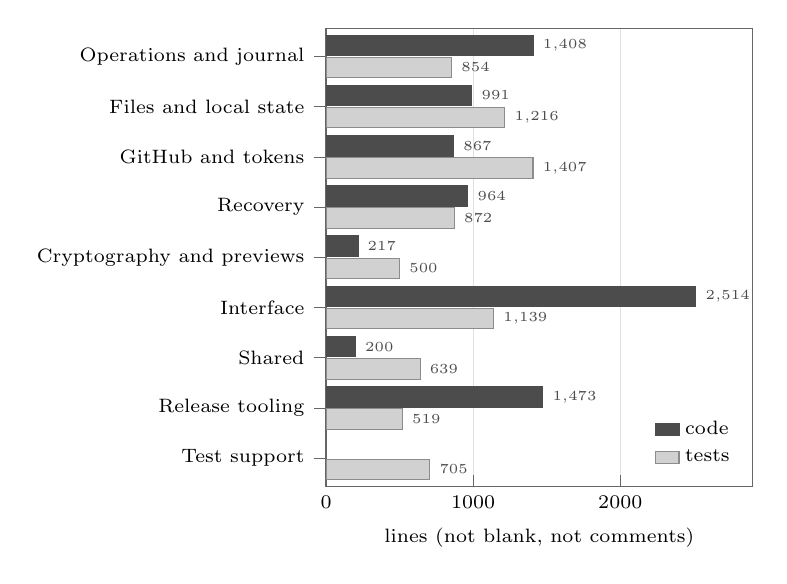
\begin{tikzpicture}
\begin{axis}[
  xbar=0.6pt, width=70mm, height=74mm,
  font=\scriptsize,
  bar width=2.6mm,
  xmin=0, xmax=2900, xtick={0,1000,2000}, xticklabels={0,1000,2000},
  scaled x ticks=false,
  xlabel={lines (not blank, not comments)},
  y dir=reverse, ytick=data, enlarge y limits=0.07,
  symbolic y coords={Operations and journal, Files and local state, GitHub and tokens, Recovery,
                     Cryptography and previews, Interface, Shared, Release tooling, Test support},
  yticklabel style={align=right},
  axis line style={black!60}, tick style={black!60},
  xmajorgrids, grid style={black!12},
  legend style={font=\scriptsize, draw=none, at={(0.98,0.02)}, anchor=south east, cells={anchor=west}},
  reverse legend,
  legend image code/.code={\draw[#1] (0mm,-0.8mm) rectangle (3mm,0.8mm);},
  xtick pos=bottom, ytick pos=left,
  nodes near coords, nodes near coords style={font=\tiny, text=black!70},
  every node near coord/.append style={anchor=west},
]
\addplot[fill=black!18, draw=black!45] coordinates {
  (854,Operations and journal) (1216,Files and local state) (1407,GitHub and tokens) (872,Recovery)
  (500,Cryptography and previews) (1139,Interface) (639,Shared) (519,Release tooling) (705,Test support)};
\addlegendentry{tests}
\addplot[fill=black!70, draw=black!70] coordinates {
  (1408,Operations and journal) (991,Files and local state) (867,GitHub and tokens) (964,Recovery)
  (217,Cryptography and previews) (2514,Interface) (200,Shared) (1473,Release tooling)};
\addlegendentry{code}
\end{axis}
\end{tikzpicture}
